\documentclass[10pt]{article}
\usepackage[margin=0.62in]{geometry}
\usepackage{times}
\usepackage{xcolor}
\definecolor{link}{HTML}{1A56B0}
\definecolor{accent}{HTML}{0B3D91}
\usepackage[colorlinks=true,urlcolor=link,linkcolor=link]{hyperref}
\usepackage{booktabs}
\usepackage{titlesec}
\usepackage{parskip}
\usepackage{pgfplots}
\pgfplotsset{compat=1.17}
\setlength{\parskip}{3pt}
\titlespacing{\section}{0pt}{5pt}{1pt}
\titleformat{\section}{\normalfont\normalsize\bfseries\color{accent}}{}{0em}{}
\pagestyle{empty}

% shorthand for a file link on GitHub
\newcommand{\gh}[1]{\href{https://github.com/neelTheCoder/nfl-big-data-bowl-2026/blob/main/#1}{\texttt{#1}}}

\begin{document}

\begin{center}
{\LARGE\bfseries\color{accent} Predicting Players in Motion}\\[1pt]
{\normalsize NFL Big Data Bowl 2026, Prediction track \;\textbullet\; Neel Ahuja}\\[2pt]
{\small \href{https://github.com/neelTheCoder/nfl-big-data-bowl-2026}{Code on GitHub} \quad\textbullet\quad \href{https://www.kaggle.com/code/neel999/nfl-bdb26-submit}{Kaggle submission notebook}}
\end{center}
\vspace{-3pt}
\hrule
\vspace{4pt}

Given every player's tracking data up to the moment the ball is thrown, predict where the
targeted players will be for each frame until it lands, scored by RMSE on the $(x,y)$
coordinates. Training is the 2023 season; the hidden test is a \emph{later} season, and that
gap is the whole story. Lower RMSE is better; a constant-velocity baseline scores 1.645.

\section*{The model}
A compact CNN$+$Transformer, roughly 1.4M parameters to start and 4.9M at full size
(\gh{train.py}). Each of the 22 players becomes one token: a \textbf{depthwise 1-D CNN}
reads that player's last 20 frames (position, speed, acceleration, heading and orientation as
sine/cosine, and vectors to the ball's landing spot and the intended receiver). A
\textbf{pre-norm SwiGLU Transformer} then lets the tokens attend across each other, since a
defender's path depends on the receiver's, and a convolutional head decodes each into a
per-frame displacement plus its own variance out to 48 frames. Training uses a Gaussian
negative-log-likelihood (the model predicts its own error bars) with velocity and acceleration
auxiliary heads, heavy geometric augmentation (random rotation, mirroring, early starts), EMA
weight averaging, and a horizontal-flip test-time average.

\section*{Autoresearch: tuning as an experiment loop}
Rather than hand-tune, I ran the project as a Karpathy-style autoresearch loop.
\gh{prepare.py} is \emph{frozen}: it builds the data and defines the RMSE metric and the
validation split, so nothing I optimize can quietly change how it is judged. \gh{train.py} is
the only file I edit, each run gets a fixed wall-clock budget so two experiments are
comparable, and every result is re-scored from saved predictions and logged with its git commit
to \gh{results.tsv}. Twelve overnight hours produced \textbf{33 tracked experiments}. The
biggest lever it found: the published recipe over-weights the velocity/acceleration loss for my
training budget, so cutting that weight and raising the learning rate alone moved the model from
0.94 to 0.63.

\section*{From holdout to leaderboard}
My champion scored 0.478 on held-out weeks but 0.579 on the real test, because the holdout was
later weeks of the \emph{same} 2023 season while the test is a new one. So I pointed the loop at
the leaderboard itself, treating each submission as a labeled data point, and swept the levers
that move an RMSE like this: learning rate, model width and depth, the auxiliary-loss weight,
augmentation, the decoder, and the ensemble makeup. Scaling to full size and 37k steps took a
single model to 0.536, and fold ensembling to 0.534. The largest jump was not a hyperparameter:
a parity test replayed raw plays through the submission path and the local scorer, they
disagreed by 0.05, and the diff showed one feature (frames-to-predict) was zeroed for every
unscored player at inference. Fixing that single line dropped the identical ensemble to 0.475.

\begin{center}
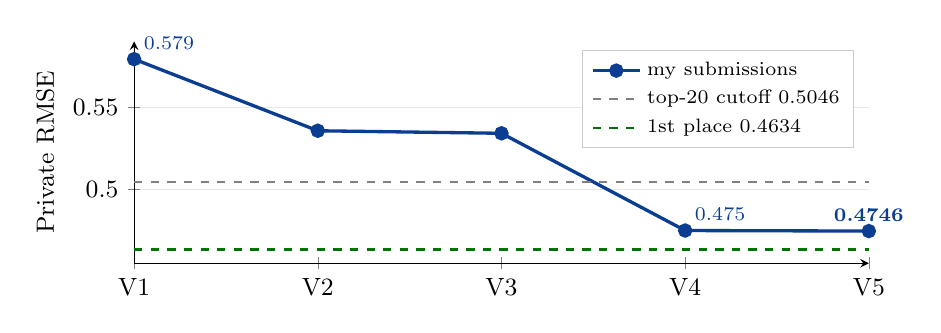
\begin{tikzpicture}
\begin{axis}[
    width=0.90\linewidth, height=4.4cm,
    ylabel={Private RMSE}, ylabel style={font=\small},
    xtick={1,2,3,4,5}, xticklabels={V1,V2,V3,V4,V5},
    tick label style={font=\small},
    ymin=0.455, ymax=0.590, ymajorgrids, grid style={gray!18},
    enlarge x limits=0.10, axis lines=left, clip=false,
    legend style={font=\scriptsize, at={(0.98,0.96)}, anchor=north east, draw=gray!40},
    legend cell align=left,
]
\addplot[color=accent, very thick, mark=*, mark options={fill=accent}]
  coordinates {(1,0.57915)(2,0.53559)(3,0.53405)(4,0.47490)(5,0.47458)};
\addlegendentry{my submissions}
\addplot[gray, dashed, thick, domain=1:5]{0.50460}; \addlegendentry{top-20 cutoff 0.5046}
\addplot[green!45!black, dashed, thick, domain=1:5]{0.46340}; \addlegendentry{1st place 0.4634}
\node[anchor=south west, font=\scriptsize, accent] at (axis cs:1,0.57915) {0.579};
\node[anchor=south west, font=\scriptsize, accent] at (axis cs:4,0.47490) {0.475};
\node[anchor=south, font=\scriptsize, accent] at (axis cs:5,0.47458) {\textbf{0.4746}};
\end{axis}
\end{tikzpicture}\\[-1pt]
{\small Five submitted versions; the drop at V4 is the inference-bug fix. Lower is better.}
\end{center}

\section*{The final model}
A four-way ensemble of the full network, each 4.9M parameters (64 channels per feature, a
256-wide 3-layer Transformer) trained on a different 2023 fold. Three members integrate
per-frame displacements and one uses the direct head, which decorrelates their errors; each is
averaged with its own flip and its own normalization. Final private RMSE \textbf{0.47458},
inside the top-20 cutoff of 0.5046 and about 0.011 off the winning 0.4634. What remains is
single-model quality, not ensembling: the next steps are full-data training with no held-out
fold and rotational test-time augmentation.

\end{document}
